\documentclass{article}
\usepackage{tikz}
\usepackage[margin=2cm]{geometry}
\pagestyle{empty}
\begin{document}
\section*{Conservative drawing damage}
Editing this sentence. The unchanged plot below should not be rasterized again
when only these words change. Reflow must move its drawing bounds correctly.

\begin{center}
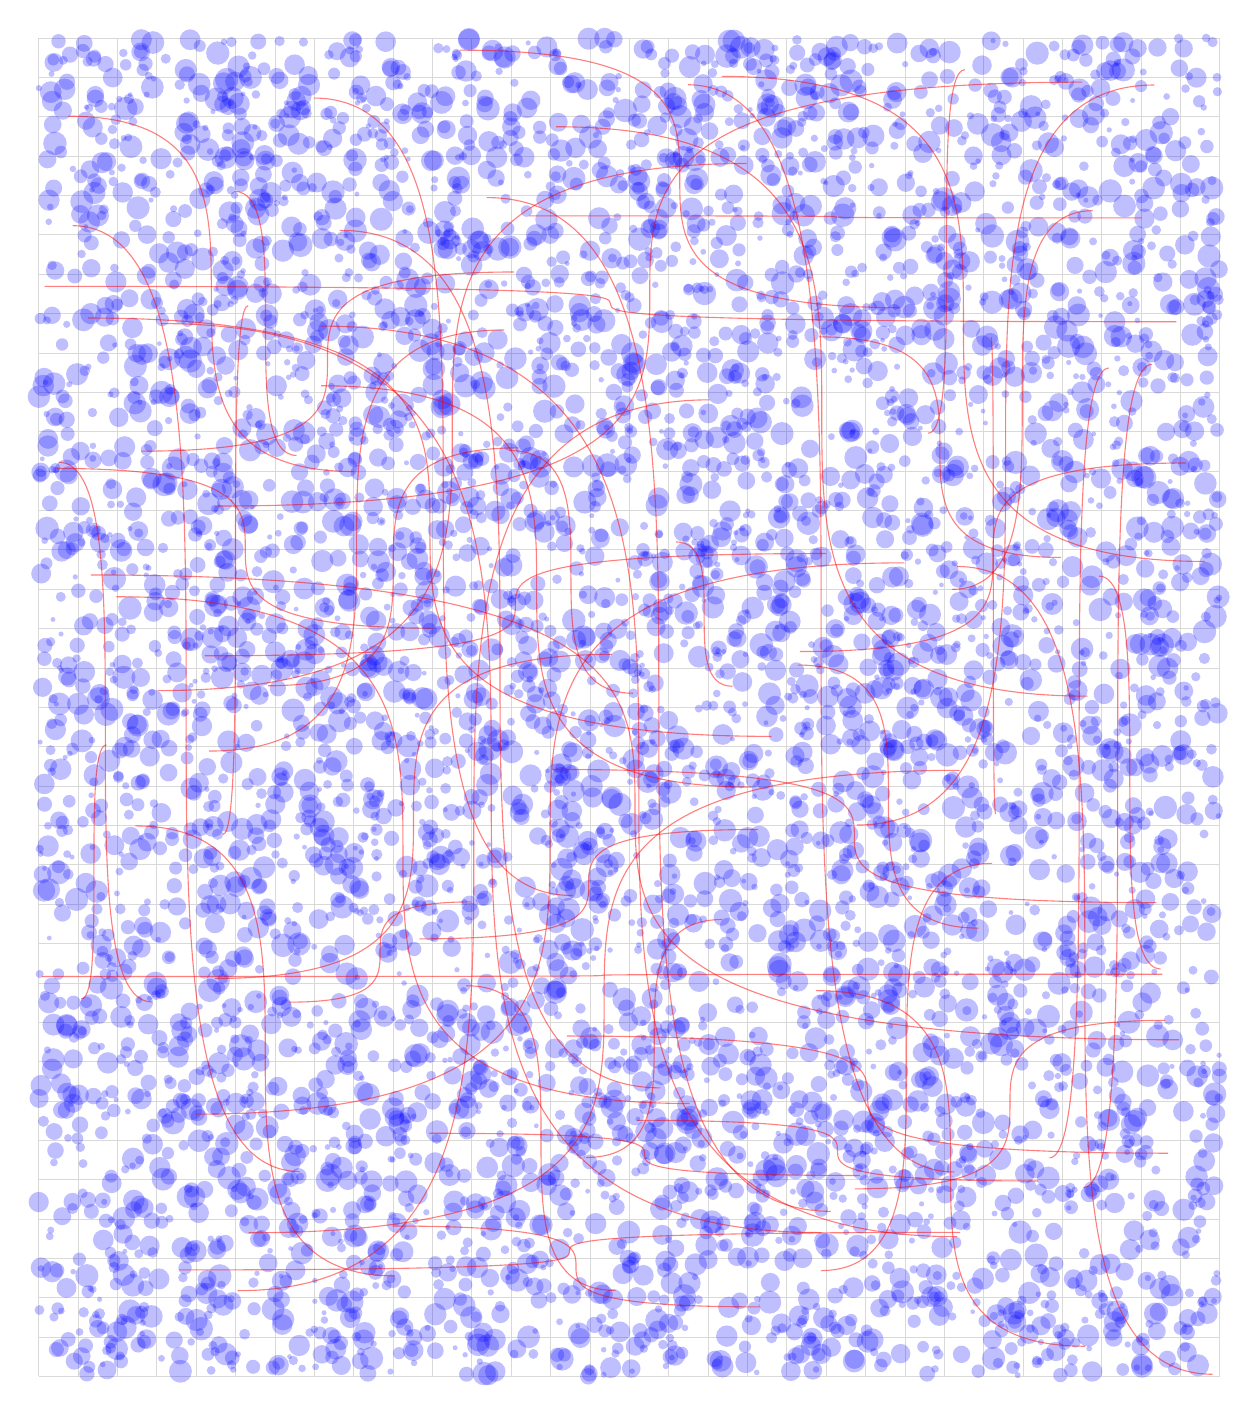
\begin{tikzpicture}
\pgfmathsetseed{7}
\draw[step=0.5,gray!30,very thin] (0,0) grid (15,17);
\foreach \i in {1,...,6000} {
  \pgfmathsetmacro\x{rnd*15}
  \pgfmathsetmacro\y{rnd*17}
  \pgfmathsetmacro\r{0.03+rnd*0.12}
  \fill[blue,opacity=0.25] (\x,\y) circle (\r);
}
\foreach \i in {1,...,60} {
  \pgfmathsetmacro\a{rnd*15}
  \pgfmathsetmacro\b{rnd*17}
  \pgfmathsetmacro\c{rnd*15}
  \pgfmathsetmacro\d{rnd*17}
  \draw[red,opacity=0.5,thin] (\a,\b) .. controls (\c,\b) and (\a,\d) .. (\c,\d);
}
\end{tikzpicture}
\end{center}
\end{document}
